\documentclass[11pt]{beamer}
\usetheme{Boadilla}
\usepackage[utf8]{inputenc}
\usepackage{amsmath}
\usepackage{amsfonts}
\usepackage{amssymb}
\graphicspath{{../fig/}}
%\author{}
\title{Updates on the new implementation of LPM effect}
%\setbeamercovered{transparent} 
%\setbeamertemplate{navigation symbols}{} 
%\logo{} 
%\institute{} 
%\date{} 
%\subject{} 
\begin{document}

\begin{frame}
\titlepage
\end{frame}

%\begin{frame}
%\tableofcontents
%\end{frame}

\begin{frame}{Status of the paper}
Main points:
\begin{itemize}
\item Model uncertainties obscure the interpretation of the extracted $\hat{q}$. \\(Is the theory favored/disfavored?)
\item A major one comes from the approximated Monte-Carlo-LPM effect $\rightarrow$ dominant at high energy.
\item We ``find" a MC approach that well reproduces the theory.
\item ``Running $\alpha_s$", ``Mass effect", ``expanding medium" are implemented.
\item It is tunable and can be applied to future calibrations.
\end{itemize}
\end{frame}

\begin{frame}{Compare Monte Carlo implementation to analytic $dE/dx$}
\begin{itemize}
\item Old approach deviates from analytic solution by $\ln(C/\alpha_s)$
\item Block radiation is not a good one! Deviate by $\alpha_s$.
\item "New" approach has the right scaling: $\alpha_s^2 E^{1/2} T^{3/2}$
\end{itemize}
\begin{center}
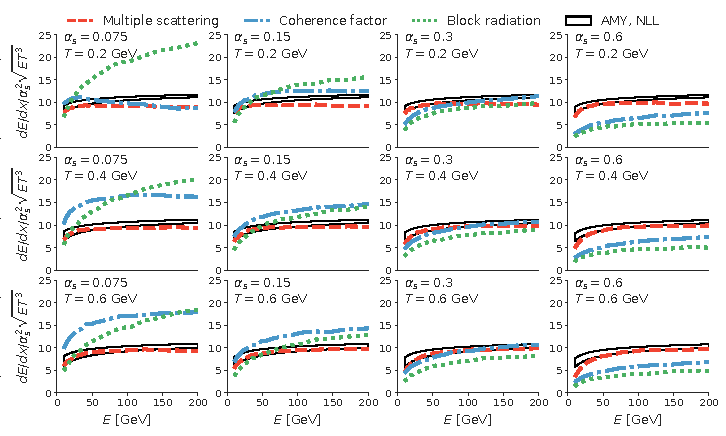
\includegraphics[width=.85\textwidth]{Eloss_infinite.pdf}
\end{center}
\end{frame}

\begin{frame}{Compare Monte Carlo implementation to analytic $\Delta E(L)$}
\begin{itemize}
\item Old approach deviates from analytic solution by $\ln(C/\alpha_s)$
\item Block radiation is not a good one! Deviate by $\alpha_s$.
\item "New" approach has the right scaling: $\alpha_s^2 E^{1/2} T^{3/2}$
\end{itemize}
\begin{center}
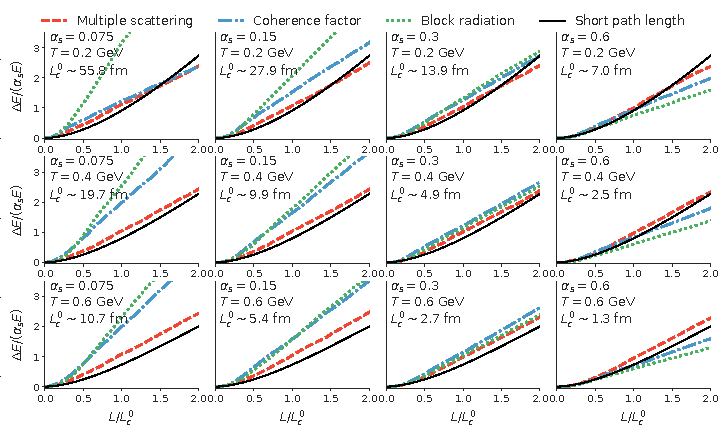
\includegraphics[width=.85\textwidth]{Eloss_Ldep.pdf}
\end{center}
\end{frame}

\begin{frame}{Compare Monte Carlo to spectrum $dI/d\omega$}
\begin{columns}
\begin{column}{.5\textwidth}
\begin{center}
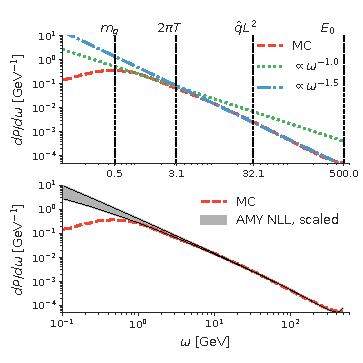
\includegraphics[width=\textwidth]{spectrum.pdf}
\end{center}
\end{column}
\begin{column}{.5\textwidth}
A strong test!\\
At asymptotic high energy
\begin{itemize}
\item $m_g<\omega<2\pi T$ reproduces the incoherent limit $\propto\omega^{-1}$.
\item $2\pi T<\omega<E$ reproduces the LPM limit $\propto\omega^{-3/2}$.
\end{itemize}
\end{column}
\end{columns}
\end{frame}


\end{document}